\newpage
\section{Discussion}
\label{sec:discussion}
\subsection{Crossmatching}
\label{sec:disc_crossmatching}
Evidently from \cref{sec:coordinate_calibration}, the crossmatching of HPICxLIFEcat with either NEA or EMC should be understood as successful and can be reasonably viewed as very close to perfectly reliable (i.e. bearing no false positives (FPs)) and complete (i.e. missing no planets)\footnote{completeness was given in the ID-matched samples; we are extrapolating from that to the entire catalog.}. Furthermore, the crossmatching is easily reproducible and update-able on any changes to NEA, EMC or HPICxLIFEcat. 
However, as mentioned in \cref{par:density_calc}, the coordinate-crossmatching radii of $r_0= 10'', r_{\text{default}} = 50''$ is orders of magnitudes larger than other crossmatching programs. By the rough calculation in that section we can argue, the lower the search radii, the lower the expected chance of FPs coordinate matching, but the radii were chosen to be the minimal ones yielding completeness. Multiple ways of achieving smaller search radii while keeping completeness are imaginable: Using the similar coordinate epochs (lower $\Delta t$), which is of note in NEA as there the epochs of some entries lie in the 1950s. For EMC, a knowledge of the proper motion of the host stars would allow significantly smaller search radii, but that is a property that is currently not tracked. 
Note also that the choice of $r_{\text{default}} = 50''$ currently is on poor footing regardless of its size, as our rough theoretical calculations do not prefer it over any value on the same order of magnitude. and the crossmatching methods still work with similar values (40'', 60'') without producing false positives. Currently the only advantage is that 50'' coincidentally produces completeness and reliability for both NEA and EMC, but that is not to say there could be other, catalog dependent choices of $r_{\text{default}}$, that hold up better for higher on-sky densities. With, ID-matching dominating its precise value is not of much importance, however if having a coordinate-only catalog at hand or similar situation, this is a quantity that should be looked at in significantly more detail.
\begin{wrapfigure}[15]{r}{0.5\linewidth}
    \centering
    \vspace{-0.75\baselineskip}
    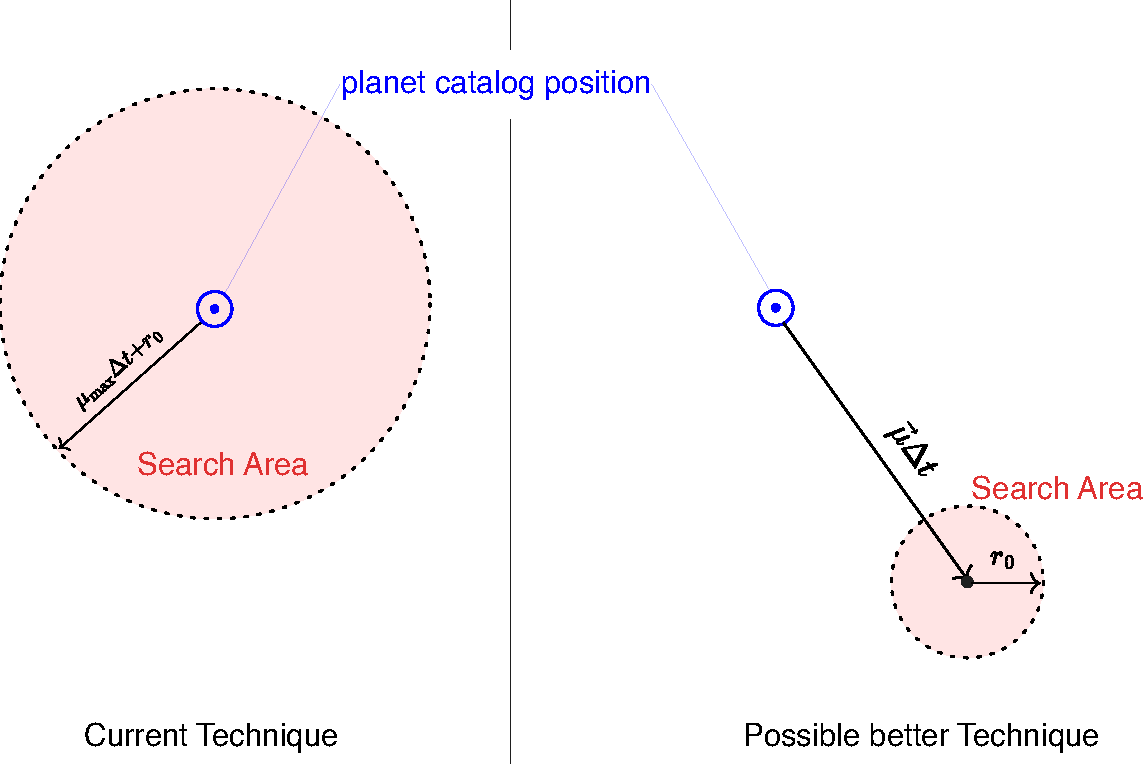
\includegraphics[width=1\linewidth]{figures/better_coordinate_matching_technique.pdf}
    \caption{Sketch of a proposed improved technique of coordinate matching for planetary catalogs (NEA falls into this category, but not EMC)}
    \label{fig:cooridnate_matching_technique}
\end{wrapfigure}
Further, for planetary catalogs, the technique could be improved (in the sense of yielding lower FP chances) on the side of this program by matching in a small area around an offset (by proper motion) position instead of the current method of tracing a circle with a radius determined by the proper motion as sketched in \cref{fig:cooridnate_matching_technique}.
Note the difference in average crossmatching distances in \cref{sec:coordinate_calibration} likely relates to the fact that Exo-MerCat takes its coordinates from SIMBAD, and so does LIFEcat, which informs part of the HPICxLIFEcat dataset. Further, HPIC's coordinates are sourced from TIC v8 \cite{hpic} and Gaia DR3, the latter of which is also used to compute some of SIMBADs entries \cite{Simbad}. In opposition, NEA carries its own heterogeneously sourced coordinate entries, many of which do not even carry the same epochs and sometimes reach back to the mid 20th century and are a priori unconnected to SIMBAD coordinates. For HPICxLIFEcat, this means that matching with EMC is preferred in view of long term avoidance of false positives. In the future, if a new catalog is assembled in a similar manner, ensuring the coordinate source (in the case of SIMBAD, also epochs) are chosen to match with the target planetary catalog (like EMC) will lower the needed search radius and thus keep the false positive occurrence rates low.
\subsection{Parameter Enrichment}
As mentioned in \cref{sec:enrichment}, the computed parameters should generally be dealt with a great deal of caution. There are multiple reasons: firstly, the combination of differently sourced data might produce unphysical results, secondly, some of the computations involve empirical-statistical relations which can admit strong outliers. Still, for a broad overview of the population as aimed for in this report, they help to show general trends.
Comparing \cref{fig:pop_distr_nocomp} (only published parameters) with \cref{fig:pop_distr} (includes computed parameters), we notice that the most extreme points come from candidate planets which typically have less trustable published parameters than confirmed planets. Furthermore, bunching appears around $\qty{E1}{\Rearth}$, which is a consequence of the \textcite{ChenKipping2017} power law's transition around that value used to estimate radii when missing \cite{NasaExoplanetArchive}. Since a large region of (minimum) mass space maps to the region close to $\qty{E1}{\Rearth}$ in radius space and many planets are known in that mass regime, they bunch around that value. By comparison of the two figures, we conclude the insolation flux values in that vertical line are mostly computed. They come only from directly imaged planets, which tend to have large separations (very low  computed insolation) and are rarely published with insolation estimation. The exact location of these data points is thus to be treated with a high amount of skepticism, but their locations are again indicative of a general trend.
\subsection{Population and its implication for LIFE}
The change in host star population in  \cref{sec:population_analysis} between the Exo-MerCat and HPICxLIFEcat stars is qualitatively in agreement with the Malmquist bias \cite{1922MeLuF.100....1M}, which is expected, as one of the main inclusion criteria for HPICxLIFEcat is a distance of less than $\qty{50}{pc}$. More complicated selection criteria determine the HPIC and LIFEcat stars, but the distance cut is the dominant effect on the stellar host population in the broader sense. This macroscopic change in the host star population qualitatively explains the differences between the HPICxLIFEcat and Exo-MerCat planet populations seen in \cref{fig:pop_heatmap}:  
\begin{itemize}
    \item The feature of hot Jupiters (upper right quadrant) is absent in the HPICxLIFEcat population; This is consistent with low-mass stars, which occupy a larger share of the host star  population in HPICxLIFEcat, being known to only rarely host hot Jupiters \cite{Ganetal2023}.
    \item The shift to on average lower insolations and radii in the HPICxLIFEcat sample is consistent with observation bias against high periods and against low $R_p/R_*$ ratios \cite{Guyon2017}. Therefore, lower mass (and thus radius) stars---which comprise a larger share of that sample compared to EMC---are more likely to have exoplanets with lower radii detected around them than their more massive counterparts.  
    \item The share of habitable planets in the HPICxLIFEcat sample can be explained in the same manner
\end{itemize}
As this only touches on the most obvious features unrigorously, a deeper and more quantitative analysis of the differences of population could be covered in future work. 
\\ \\
Note also that in either population, no  planets are excluded from being classified as temperate and rocky by having suitable insolation values and less than $0.5\Rearth$. This is likely due to observational biases against low-mass/radius and comparatively long-period planets \cite{Guyon2017}, hinting that with better telescopes, those parts of phase space may feature more planets.
The population differences can be viewed with cautious optimism, as this means that the chosen set of stars is more likely than average to host known habitable exoplanets. This forms a strong argument for the chosen mission specifications, specifically wavelength ranges, for LIFE.
However, it would be somewhat premature to conclude that this means low-luminosity and very-low-luminosity stars host more habitable planets than their higher mass counterparts because, in general, it is not known which features of the known exoplanet population are attributable to observational bias and which are "fundamental". This disentanglement is the focus of statistical surveys that compare the observed population with the currently accepted theory \cite{exoStats}. Theoretical predictions of LIFE yield goes beyond the scope of this project, thus we only proclaim a better-than average habitability chance with respect to the \textit{known} planet population.
\subsection{Outlook}
This project stands as a tool to quickly and reliably match known exoplanets to any stellar catalog and determine its habitable subpopulation, which can be used in the future for yield estimates similar to how a simulated exoplanetary catalog was employed by \textcite{life4}. Furthermore, this work may be used for studies similar to \citetitle{Life10} by \textcite{Life10} by providing a quick and repeatable way of selecting potentially habitable planets to then study on a case by case basis, which may inform the characterization phase target list.
Crossmatching performance, especially the certainty that we do not have false positive matches, could be improved by augmenting Exo-MerCat with a proper motion data sourcing or by implementing an algorithm taking into account the proper motion in the stellar catalog and by implementing more robust matching techniques as sketched in \cref{sec:disc_crossmatching} .
On the enrichment side, searching for more published empirical and physical relations of stars and planets could lead to more sophisticated enrichment pathways, which further increases the number of inferred parameters. Simultaneously, adding more data sources (for example, Gaia DR3 as done in \cite{Bohl_2026}) could lead to an even better understanding of the broader known exoplanet population. 
By adopting some of \citetitle{Bohl_2026} by \textcite{Bohl_2026} methods---specifically the more intricate calculation of the habitable zones using polynomials with stellar temperature,  including eccentricity in the planet insolation considerations and their estimates of stellar age and its implication for the evolution of life---while using the larger dataset of Exo-MerCat could lead to a potentially different and more detailed understanding of the HPICxLIFEcat planet population or any catalogs habitable planet population for LIFE target selection. 
